% !TeX spellcheck = fr_FR
\chapter{Chapitre 3 : Architecture de l'application et implémentations}

L'application produite lors de ce travail de bachelor se base sur une implémentation existante de certains outils réalisés lors d'un projet de semestre. Elle est principalement réaliser dans le langage de programmation Rust qui est un langage moderne mutiparadigme, fiable, rapide et sécurisé au niveau de la mémoire. Rust utilise des outils dédiés au langage pour accélérer le développement de logiciels dont "cargo" qui est un gestionnaire de paquet et de compilation, "rustdoc", un générateur de documentation à partir du code source et "clippy", un analyseur de code qui indique des erreurs communes réalisées lors de l'écriture du code. 

Dans la nomenclature de Rust, le mot "crate" désigne un paquet ou une librairie externe. Une particularité de Rust est le \textbf{ownership} ou la propriété des données. C'est grâce à ce principe que l'on peut avoir une mémoire sécurisé contre les fuites mémoires ou dans des logiciels multithreadés une absence de datarace.

\section{Architecture}
L'application est composée de quatre modules principaux.
La librairie qui regroupe les fonctions et les structures qui sont communes à l'application.
Le serveur expose les fichiers mis à disposition par le \gls{sitg} au travers d'un binaire dédié.
Le client web servant de visualiseur de donnée pour un utilisateur étant aussi un binaire et
les utilitaires, contenant les entrées des programmes utilitaires en ligne de commande telle que la triangulation d'un fichier lidar ou encore la triangulation de plusieurs régions ensemble.

\section{Librairie}

La librairie contient les outils de lecture et d'écriture de fichiers pour les formats du chapitre 2. Elle expose aussi les structures de données pour les différents algorithmes du chapitre 2.

Elle a comme dépendance principale les crates "stl-io" qui implémentes les structures pour écrire les fichiers \gls{stl} et "las-rs" qui expose les structures et méthodes liées aux données lidar.

\begin{figure}[htbp!]
    \centering
    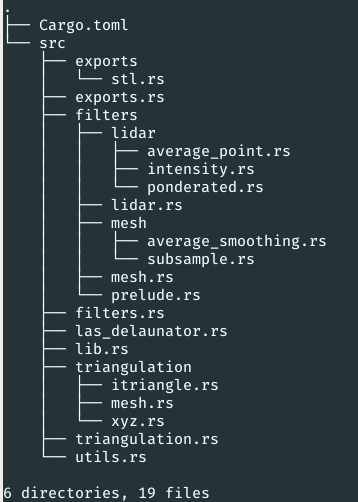
\includegraphics[width=0.5\linewidth]{figures/architecture.png}
    \caption{Structure de fichier présent dans le module de la librairie de l'application. Source : réalisé par Jérôme Chételat}
    \label{fig:library_tree}
\end{figure}

\subsection{Filtres}
Les implémentations des filtres sont dérivées du trait \textbf{MeshFilter} ou du trait \textbf{LidarFilter}. Leurs définitions sont les suivantes :
\begin{lstlisting}[language=Rust, style=boxed]
pub trait MeshFilter {
    fn apply(&self, mesh: IndexedMesh, epsilon: f32) -> IndexedMesh;
}

pub trait LidarFilter {
    fn apply(&self, points: Vec<Point>) -> Vec<Point>;
}

\end{lstlisting}

Les traits sont ensuite spécialisé dans le type de filtre voulu
\subsection{Triangulation}
La librairie contient un module de triangulation.
On y trouve les implémentations des algorithmes de triangulation réalisés lors du projet de semestre et de fusion de triangulation.

\subsection{Fusion de triangulation}
Pour ce qui est de la fusion, une structure propre à la librairie était nécessaire en plus des structures de données offertes par la crates stl-io.
Elle est définie de la manière suivante:
\begin{lstlisting}[language=Rust, style=boxed]
pub struct Mesh {
    /// Vertices composing the mesh
    pub vertices: Vec<XYZ>,
    /// Indexed triangles of the mesh
    pub faces: Vec<usize>,
    /// Indexed vertices part of the convex hull of the mesh
    pub hull: Option<Vec<usize>>,
    /// The neighbourhood of each indexed point
    pub neighbourhood: Option<Vec<HashSet<usize>>>,
}
\end{lstlisting}

On y trouve notamment un champ pour le voisinage du maillage qui est "neighbourhood" et son enveloppe convexe dans le champ "hull".
Ils sont optionnels pour maintenir une compatibilité avec les crates utilisées dans la librairie.
Une des raisons vient du fait que lors de la lecture d'un fichier \gls{stl}, on ne retrouve pas ces champs. 

Une méthode utile pour s'assurer de la présence d'un voisinage est d'appeler la fonction neighbourhood. Elle renvoie le voisinage d'un maillage s'il est déjà présent, le cas échéant est de calculer les voisins.

Voici l'implémentation : 
\begin{lstlisting}[language=Rust, style=boxed]
pub fn neighbourhood(&mut self) -> Option<Vec<HashSet<usize>>> {
        if self.neighbourhood.is_some() {
            return self.neighbourhood.clone();
        }
        let mut dict: Vec<HashSet<usize>> = 
            vec![HashSet::new(); self.vertices.len()];

        // Iterating over all triangles in the mesh
        self.faces
            .iter()
            .enumerate()
            .step_by(3)
            .for_each(|(i, _): (usize, &usize)| {
                // Adding the neibours of the first vertex
                dict[self.faces[i]].insert(self.faces[i + 1]);
                dict[self.faces[i]].insert(self.faces[i + 2]);

                // Adding the neibours of the second vertex
                dict[self.faces[i + 1]].insert(self.faces[i]);
                dict[self.faces[i + 1]].insert(self.faces[i + 2]);

                // Adding the neibours of the third vertex
                dict[self.faces[i + 2]].insert(self.faces[i]);
                dict[self.faces[i + 2]].insert(self.faces[i + 1]);
            });

        self.neighbourhood = Some(dict.clone());
        Some(dict)
}
\end{lstlisting}

Elle parcourt les différents triangles du maillage et pour chaque point présent du triangle, on ajoute ses deux voisins dans une liste.

Concernant le champ hull, il est possible de le calculé au travers de la crate "ncollide" qui expose une version de quickhull, un algorithme de calcule d'enveloppe convexe.

La première est la recherche d'un candidat final dans un maillage. Voici la signature de la fonction:
\begin{lstlisting}[language=Rust, style=boxed]
fn get_side_candidate(
        mesh: &mut Mesh,
        lr_indexed_point: usize,
        other_lr_point: &XYZ,
    ) -> Option<usize>;
\end{lstlisting}

Elle prend en paramètre un point indexé par un entier non signé dans le maillage passé en argument et une structure de point pour effectuer la recherche et retourne éventuellement un index pour le site choisi.

Une grosse partie de la fusion est réalisée dans la méthode \textbf{merge} avec comme signature : 
\begin{lstlisting}[language=Rust, style=boxed]
/// Returns a Ok(Mesh) containing the fusion of two meshes togheter.
/// It needs the convex hull of each mesh.
pub fn merge(&mut self, other: &mut Mesh) -> Result<Mesh, &'static str>;
\end{lstlisting}

La méthode renvoie un maillage dans le cas où toute la fusion s'est bien déroulée sinon elle renvoie un message d'erreur.

Une partie intéressante de la l'implémentation est la création des arêtes entre la base et un candidat.

\begin{lstlisting}[language=Rust, style=boxed]
loop {
    let candidate_right = Mesh::get_side_candidate(
        other,
        r_bs,
        &self.vertices[l_bs]);
    let candidate_left = Mesh::get_side_candidate(
        self,
        l_bs,
        &other.vertices[r_bs]);
    let candidates = (candidate_left, candidate_right);
    match candidates {
        (Some(l), Some(r)) => {
            // Check that one of these does not contain the other one
            let left_candidate_inside = self
                                            .vertices[l]
                                            .inside_circum_circle((
                                                &self.vertices[l_bs],
                                                &other.vertices[r_bs],
                                                &other.vertices[r],
                                            ));
            let right_candidate_inside = other
                                            .vertices[r]
                                            .inside_circum_circle((
                                                &self.vertices[l],
                                                &self.vertices[l_bs],
                                                &other.vertices[r_bs],
                                            ));
            match (left_candidate_inside, right_candidate_inside) {
                // If both are contained in each other
                // it is a degenerate case and there
                // is no possible outcome
                // to have a good Delaunay triangulation
                (false, false) => 
                        return Err(
                        "Edge case found about 4 co-circular points"
                        ),
                (true, false) => {
                    edges.push(l);
                    edges.push(r_bs);
                    l_bs = l;
                }
                (false, true) => {
                    edges.push(l_bs);
                    edges.push(r);
                    r_bs = r;
                }
                _ => break,
            }
        }
        (Some(l), None) => {
            // Connect it to the lr base,
            // push the new triangle and move the l_bs reference
            edges.push(l);
            edges.push(r_bs);
            l_bs = l;
        }
        (None, Some(r)) => {
            // Connect it to the lr base, 
            // push the new triangle and move the r_bs reference
            edges.push(l_bs);
            edges.push(r);
            r_bs = r;
        }
        _ => {
            // The merging is done if it doesn't exists anymore candidates
            break;
        }
    }
}
\end{lstlisting}

Un point intéressant est l'utilisation de pattern matching provenant de langage de programmation fonctionnel pour vérifier les conditions énumérées dans le chapitre 2.3. Si un candidat final est choisi, il est ajouté a une liste d'arrête \textbf{edges} et à la fin de l'opération, cette liste est utilisée afin de construire les nouveaux triangles entre les deux maillages.

\section{Utilitaires}

Ce module contient les différents binaire en ligne de commande pour traiter les données. Il s'agit de l'implémentation concrète des différents algorithmes de la librairie. L'implémentation en ligne de commande utilise la crate clap. Elle facilite la mise en oeuvre de la désérialization 

\section{Serveur}

Le serveur est une application binaire qui utilise le framework actix-web. Ce framework utilise les nouvelles fonctionnalités du langage telles que les async/await sur des routes. Il s'agit donc d'une \gls{api} de \gls{rest} exposant une seule route pour récupérer les fichiers de manière statique. Un futur projet pourrait construire un service de triangulation ou encore un service de filtrage.

\section{Client web}

Le client web a été écrit en Rust et compilé en \gls{wasm}. Il utilise webgl pour afficher les points et les maillages. WebPack ,un bundler de frontend, a été utilisé pour liés le HTML, le JavaScript et les modules \gls{wasm}. 

Cette partie utilise grandement une crate appelée "web-sys" qui met à disposition des bindings pour le JavaScript.
On utilise également la crate "nalgebra" qui propose des fonctions pour manipuler des matrices 4x4 utilisées dans les \gls{api} graphique.

Une contrainte parvient en écrivant du code pour le web avec Rust est que la plupart des fonctionnalités pour amélioré le fonctionnement des modules est à ce jour encore expérimentale et de ce fait pas suffisamment stable pour créer une application complète.

N'étant pas assez optimisé, l'affichage d'une région entière d'un fichier \gls{lidar} ou sa version triangulée est impossible malgré une implémentation en \gls{wasm} afin de bénéficié d'une performance supplémentaire par rapport à une version qui serait écrite en javascript.